\chapter{Work Packages}
\label{ch:WP}

\section{Translator}
\paragraph{}
In a hierarchical architecture involving different MANOs, there is a need of conversion of network descriptors to schemas of respective MANO. Service Descriptor Translator (SDT) serves the purpose of translating network descriptors, namely NSDs and VNFDs from schema of SONATA Pishahang to that of OSM and vice versa.
\paragraph{}
In a scenario, where a parent MANO, say Pishahang decides to deploy one of the network services in its lower hierarchy MANO, say OSM, the NSD and VNFD(s) need to be converted to the descriptor schema of OSM. In such an event, the Scramble plugin calls the translator service and sends the descriptors to the SDT, where the translation of the descriptors takes place and the translated descriptors are sent to Adaptor utility for deployment in appropriate MANO. Figure \ref{fig:service-descriptor-translator} gives a high level view of Translator.
\paragraph{}
Scramble plug-in installed within the parent MANO forwards the network descriptors with service request to Scramble Main-Engine. Main-Engine checks the service request and sends the network descriptors to Translator along with the information of destination schema. On receiving the network descriptors, SDT translates the same to requested schema and calls the validator function to validate the translated network descriptors. Once validation is complete, the translated descriptors will be sent to Adaptor for deployment. 




\begin{figure}
	\centering
	\includegraphics[width=1\linewidth]{"figures/Service Descriptor Translator"}
	\caption{}
	\label{fig:service-descriptor-translator}
\end{figure}

\subsection{Architecture \& Work flow}
\subsection{usage}
The Translator engine consists of the following modules:
\begin{enumerate}
	\item descriptorReader
	\item descriptorWriter
	\item utilities
	\item translator
	\item validator
	
\end{enumerate}

\subsubsection{descriptorReader}

This module is responsible to read a json/dictionary input (NSD/VNFD) and iterate over the keys and return a generator of an object to the calling program. This generator can be transformed to any python data structure for ease of use and navigation. 

The input to this module is a json or dictionary object.

\begin{lstlisting}[language=Python]
from descriptorReader import read_dict

pishahang = pishahang_descriptor ## the descriptor as a json or dict object

### reading a dict/ json content into a pandas dataframe
reader = read_dict()

pishahang_dataset = pd.DataFrame(
reader.dict_parser(pishahang,'root', 1, '0|preroot|0'), 
columns=['parent_level', 'parent_key', 'level', 'key', 'value', 'lineage'])


pishahang_dataset.sort_values(ascending=True, by=['level', 'parent_key'],inplace=True)
pishahang_dataset.fillna('NULL', inplace=True)
pishahang_dataset.reset_index(drop=True,inplace=True)

\end{lstlisting}
\subsubsection{descriptorWriter}

This module is responsible to read a python pandas Dataframe input and output a nested json/dictionary maintaining the nested structure in the dictionary.

\begin{lstlisting}[language=Python]
from descriptorWriter import write_dict

### writing from a pandas dataframe to a dict/json object
writer = write_dict()
pishahang_descriptor = writer.translate(pishahang_dataset.sort_values(by='lineage'))

\end{lstlisting}

\subsubsection{utilities}

This module is responsible for transforming the keys and map the corresponding values between sonata and osm descriptors. The module includes the 4 functions for translating between sonata and OSM descriptors. 
\begin{enumerate}
	\item translate\_to\_osm\_nsd()
	\item translate\_to\_osm\_vnfd()
	\item translate\_to\_sonata\_nsd()
	\item translate\_to\_sonata\_vnfd()
\end{enumerate}

\subsubsection{translator}

This is the interface where the actual translation request comes in. After a tranlsation request is received along with a descriptor, it calls the above modules translate and validate the descriptors (NSD/VNFD).

This following function translates OSM descriptor to sonata.
\begin{lstlisting}[language=Python]
import pymongo
from validate import validator
from utilities import setup

def toSonata(received_file):

	client = pymongo.MongoClient("mongodb://mongo:27017")
	setup_obj = setup(client)
	validate_obj = validator()
	
	if 'vnfd:vnfd-catalog' in received_file:
	
	## mongoDB document object to store the translated vnfd
	doc = setup_obj.db_descriptors["translated_vnfd"]
	
	## getting a translated sonata vnfd
	translated = setup_obj.translate_to_sonata_vnfd(received_file)
	
	## validating the translated descriptor which returns a "True"/ "False" string
	check = validate_obj.sonata_vnfd_validate(translated)
	
	if check == "True":
	## insert into mongoDB as a Document
	temp = doc.insert_one(translated)
	translated_ref = temp.inserted_id
	
	elif 'nsd:nsd-catalog' in received_file:
	
	## mongoDB document object to store the translated nsd
	doc = setup_obj.db_descriptors["translated_nsd"]
	
	## getting a translated sonata nsd
	translated = setup_obj.translate_to_sonata_nsd(received_file)
	
	## validating the translated descriptor which returns a "True"/ "False" string
	check = validate_obj.sonata_nsd_validate(translated)
	
	if check == "True"
	## insert into mongoDB as a Document
	temp = doc.insert_one(translated)
	translated_ref = temp.inserted_id
	
	return {"descriptor":translated ,"VALIDATE STATUS" :check}
\end{lstlisting}

The following function translates sonata descriptor to OSM.
\begin{lstlisting}[language=Python]
import pymongo
from validate import validator
from utilities import setup

def toOsm(received_file):

	client = pymongo.MongoClient("mongodb://mongo:27017")
	setup_obj = setup(client)
	validate_obj = validator()
	
	if 'network_functions' in received_file:
	
	## mongoDB document object to store the translated nsd
	doc = setup_obj.db_descriptors["translated_nsd"]
	
	## getting a translated osm nsd
	translated = setup_obj.translate_to_osm_nsd(received_file)
	
	## validating the translated descriptor which returns a "True"/ "False" string
	check= validate_obj.osm_validator(translated)
	
	if check == "True":
	## insert into mongoDB as a Document
	temp = doc.insert_one(translated)
	translated_ref = temp.inserted_id
	
	elif 'virtual_deployment_units' in received_file:
	
	## mongoDB document object to store the translated vnfd
	doc = setup_obj.db_descriptors["translated_vnfd"]
	
	## getting a translated osm vnfd
	translated = setup_obj.translate_to_osm_vnfd(received_file)
	
	## validating the translated vnfd which returns a "True"/ "False" string
	check= validate_obj.osm_validator(translated)
	
	if check == "True":
	## insert into mongoDB as a Document
	temp = doc.insert_one(translated)
	translated_ref = temp.inserted_id
	
	return {"descriptor":translated ,"VALIDATE STATUS" :check}
\end{lstlisting}

\subsubsection{validator}

The validator validates the descriptors presented for translation. It differentiates between OSM, Pishahang and Sonata descriptors and also between NSD's and VNFD's. The sonata descriptor validation is mainly based on schema, implemented using python library jsonschema.draft4validator, this library helps by proving the complete path of the error which comes very handy while debugging. The Validation for OSM is slightly complex than that compared to sonata validator, OSM validator can be divided into two parts. the first part validates the descriptors using schema with the same setup as that of sonata and the second part uses python object class for validation, this is done to replicate the validation method used by OSM hence to make sure that any descriptor that is validated by translator will be accepted by OSM.

\subsection{challenges}

\subsection{Future scope of this work package}

Translator engine currently doesnot support the following:
\begin{enumerate}
	\item Forwarding Graph
	\item Juju charms in OSM
	\item Monitoring Parameters
\end{enumerate}

\subsection{challenges}
\subsection{Future scope of this work package}

\section{Splitter}
Splitter helps in splitting a Network Service (NS) into multiple sub Network services which can be deployed and instantiated individually on Internet Service Providers (ISPs) located over a vast geographical region spanning multiple domains and are orchestrated by different MANO frameworks. Splitter calls Service Descriptor Transltor if there is a need to translate the NS if it is to be deployed on a different MANO framework.

In this work package, a Service Descriptor Splitter (SDS) is implemented which splits the NSD of a network service. SDS takes
NSD as an input that contains all the information elements which can be extracted to generate separate NSDs. In the proposed approach, the service graph is extracted from the input NSD
and is split into subgraphs that result in a separate NSD which includes a set of elements such as VNFs, Virtual Links (VLs), forwarding graphs of VNFs etc, according to the specific MANO
framework.
\subsection{Architecture \& Work flow}
Service Descriptor Splitter consists of following functional items which 
\begin{itemize}
	\item The total number of NFs mentioned in all the set matches the number of NFs defined in the NSD.
	\item There are no invalid NFs in the sets received.
\end{itemize}

After validation the actual splitting starts. We have created classes for different sections of a NSD which encapsulate all the attributes and its values into a single unit which makes it very easy to process. Once the objects are set they are passed to different splitting functions based on there type. We have two different processing units for OSM and SONATA. Following are some functions responsible for splitting the NSD.

\begin{itemize}
	\item \textbf{Set General information: }This function copies all the general information from the main NSD to the sub NSDs. Information includes Vendor, author, Version, Descripton etc.
	\item \textbf{Split Network Functions: }This function splits the Network functions from NSD to sub sets according to the request parameter received. 
	\item \textbf{Split Virtual Links: }When a NSD is splitted into different parts, its topology changes. Change in topology results in changing of Virtual Links. For example if A, B and C are three Nfs and we are splitting them in such a way so that A and B remain in one NSD and C in separate NSD. A virtual link between B and C now does not make sense. So this link should be broken down and B’s output should be connected to the external end point which was connected to C’s input earlier. This function splits these kind of Virtual Links.
	\item \textbf{Split Forwarding Graph: }As explained in the above section, once the topology changes, the respective Forwarding graph also changes. Split forwarding graph pulls out the set of connection points and newly created virtual links and sets them in the sub NSDs.
\end{itemize} 

Once the Splitting is done, create file is responsible for creating YAML files depending on the number of sub NSDs created. These files are saved in the file system which can be downloaded or moved forward to the adopter for deployment purpose. Following figure \ref{fig:splitter} graphically represents the splitting architecture.

\begin{figure} [h]
	\centering
	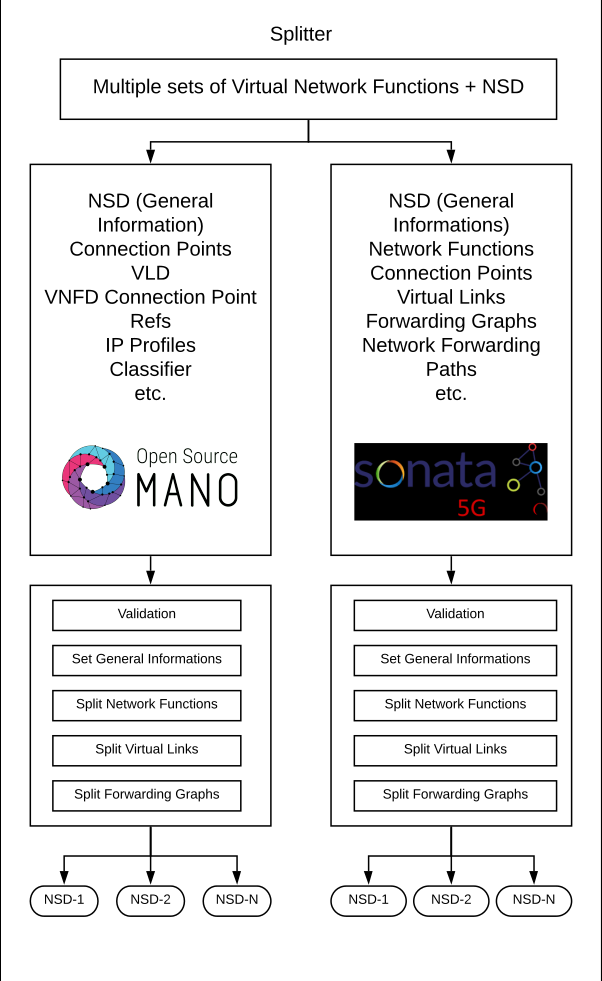
\includegraphics[width=0.5\linewidth]{figures/splitter}
	\caption{Scramble Architecture}
	\label{fig:splitter}
\end{figure}


\subsection{Usage}

SDS is implemented as a micro-service which can be used independently from Translator or Wrapper by making a post call to the SDS. Following code snippet describes how to call SDS using POST call.

\begin{lstlisting}[caption=POST call to SDS, label=lis:postSDS]

splitter_url=http://$HOST:8003/Main_splitter/split

# Body: descriptor contains NSD, vnfid_set contains set of VNF ids
nsd = { 'descriptor' : descriptor, 'sets': vnfid_set}

LOG.info("Calling Scramble Splitter..." )
response  = requests.post(splitter_url,
                          data=json.dumps(nsd_to_split))

print(response)

\end{lstlisting}

Following are some of the important functions which helps SDS in splitting the NSD with respective code snippet.

\subsubsection{Basic Python classes for NSD Schema}
\subsubsection{Splitting} "splitsonata" calls the splitting function one by one to split the list of objects created out of NSD. Following code snippet shows the sequence of function calls.

\begin{lstlisting}[caption=Sequence of function calls, label=lis:functioncalls]

    def split_sonata(self):
        if self.validate() is not False:
            self.create_new_function_sets()
            self.set_connection_point_refs_for_virtual_functions()
            self.split_network_function()
            self.set_connection_points()
            self.split_virtual_links()
            self.split_forwarding_path()
            self.set_general_information()
            return self.create_files()
        else:
            print("Validation Failed!!")

\end{lstlisting}

\subsubsection{Validate} Validate method validates the request coming from the MANOs. For example, if MANO is requesting a NSD to be split into three parts but the original NSD contains just two VNFs then the SDS will throw validation error.

\begin{lstlisting}[caption=Splitting Request Validation, label=lis:validation]

    def validate(self):
        size = 0
        list_network_function = []
        for network_function_set in self.network_function_sets:
            size = size + len(network_function_set)
            for network_function in network_function_set:
                list_network_function.append(network_function)

        if size != len(self.utilityFunctions.list_nf):
            return False
        if len(list_network_function) != len(set(list_network_function)):
            return False

\end{lstlisting}

\subsubsection{Split Network Functions}
\todo[inline]{Content to be added}
\subsubsection{Split Forwarding Graph}

\todo[inline]{Content to be added}
\subsection{Challenges}
The NSD schema of Pishahang and OSM contains a lot of elements. However the challenge we faced was choosing which elements to include for splitting. We tackled it by including mandatory elements and few optional elements from the schema which were present in the input NSD.
\subsection{Future scope of Service Descriptor Splitter}
SDS can currently split NSD of Pishahang and OSM. SDS is built in such a way that it can be implemented for MANO frameworks as well. To implement SDS for a new MANO framework one can refer the implementation of either Pishahang or OSM. First step would be to create basic python classes from the NSD schema of the MANO framework then writing the utility functions to pull the information from the NSD file and store it in the objects of the basic python classes. Lastly writing splitting functions to actually split the list of objects in two or more parts.

Also, the current implementation considers all mandatory elements and a few optional elements from a NSD schema for splitting which can be extended to include other fields (Provided they are present in the input NSD for splitting).

Current implementation of SDS can split a forwarding graph of a NSD (Pishahang) with just three VNFs. Splitting of a forwarding graph is implemented by keeping future implementation for more than three VNFs in mind (Refer Splitting of Forwarding graph section)

\section{Adaptor}

Facilitating easy communication between MANOs is an important aspect of scramble. 
Adaptor is a component that enables communication between MANOs by wrapping the REST APIs of MANOs in python code.\\

Python MANO Wrappers (PMW) is a uniform python wrapper library for various implementations of NFV Management and Network Orchestration (MANO) REST APIs. 
PMW is intended to ease the communication between python and MANO by providing a unified, convenient and standards oriented access to MANO API.\\

To achieve this, PMW follows the conventions from the ETSI GS NFV-SOL 005 (SOL005) RESTful protocols specification. 
This makes it easy to follow and the developers can use similar processes when communicating with a variety of MANO implementations.\\

PMW is easy to install, use and well documented. 
Code usage examples are available along with the detailed documentation at the following link \url{https://python-mano-wrappers.readthedocs.io/en/adaptor/}. \\

PMW is planned and released as an independent library. 
In scramble, PWM helps in inter communication of different instances of MANO, thereby creating opportunity for more advanced feature set, for example, hierarchical scaling. 
Operations such as on-boarding of NSD and VNFD, instantiation and termination of NS can be performed with ease.

\subsection{Architecture \& Work flow}
Standards based approach is a fundamental design principle behind PMW's design. 
A Common interface template is defined in compliance with SOL005 which contains the blueprint for all the methods mentioned in the standards. 
These methods are divided into different sections as per SOL005 into the following:

\begin{itemize}
	\item \textbf{auth: }Authorization API
	\item \textbf{nsd: }NSD Management API
	\item \textbf{nsfm: }NS Fault Management API
	\item \textbf{nslcm: }Lifecycle Management API
	\item \textbf{nspm: }NS Performance Management API
	\item \textbf{vnfpkgm: }VNF Package Management API
\end{itemize} 

In the figure \ref{fig:wrapperarch}, different sections of PMW are visualized. 
As part of the scramble project, support for Open Source MANO (OSM) and Sonata was implemented based on the common interface. 
This is represented by the dotted lines to OSM and Sonata modules. 
These modules are based on the common interface and implement the methods it has defined. 
Wrappers also support additional functionalities of Pishahang, which is an extension of Sonata. 

\begin{figure}
	\centering
	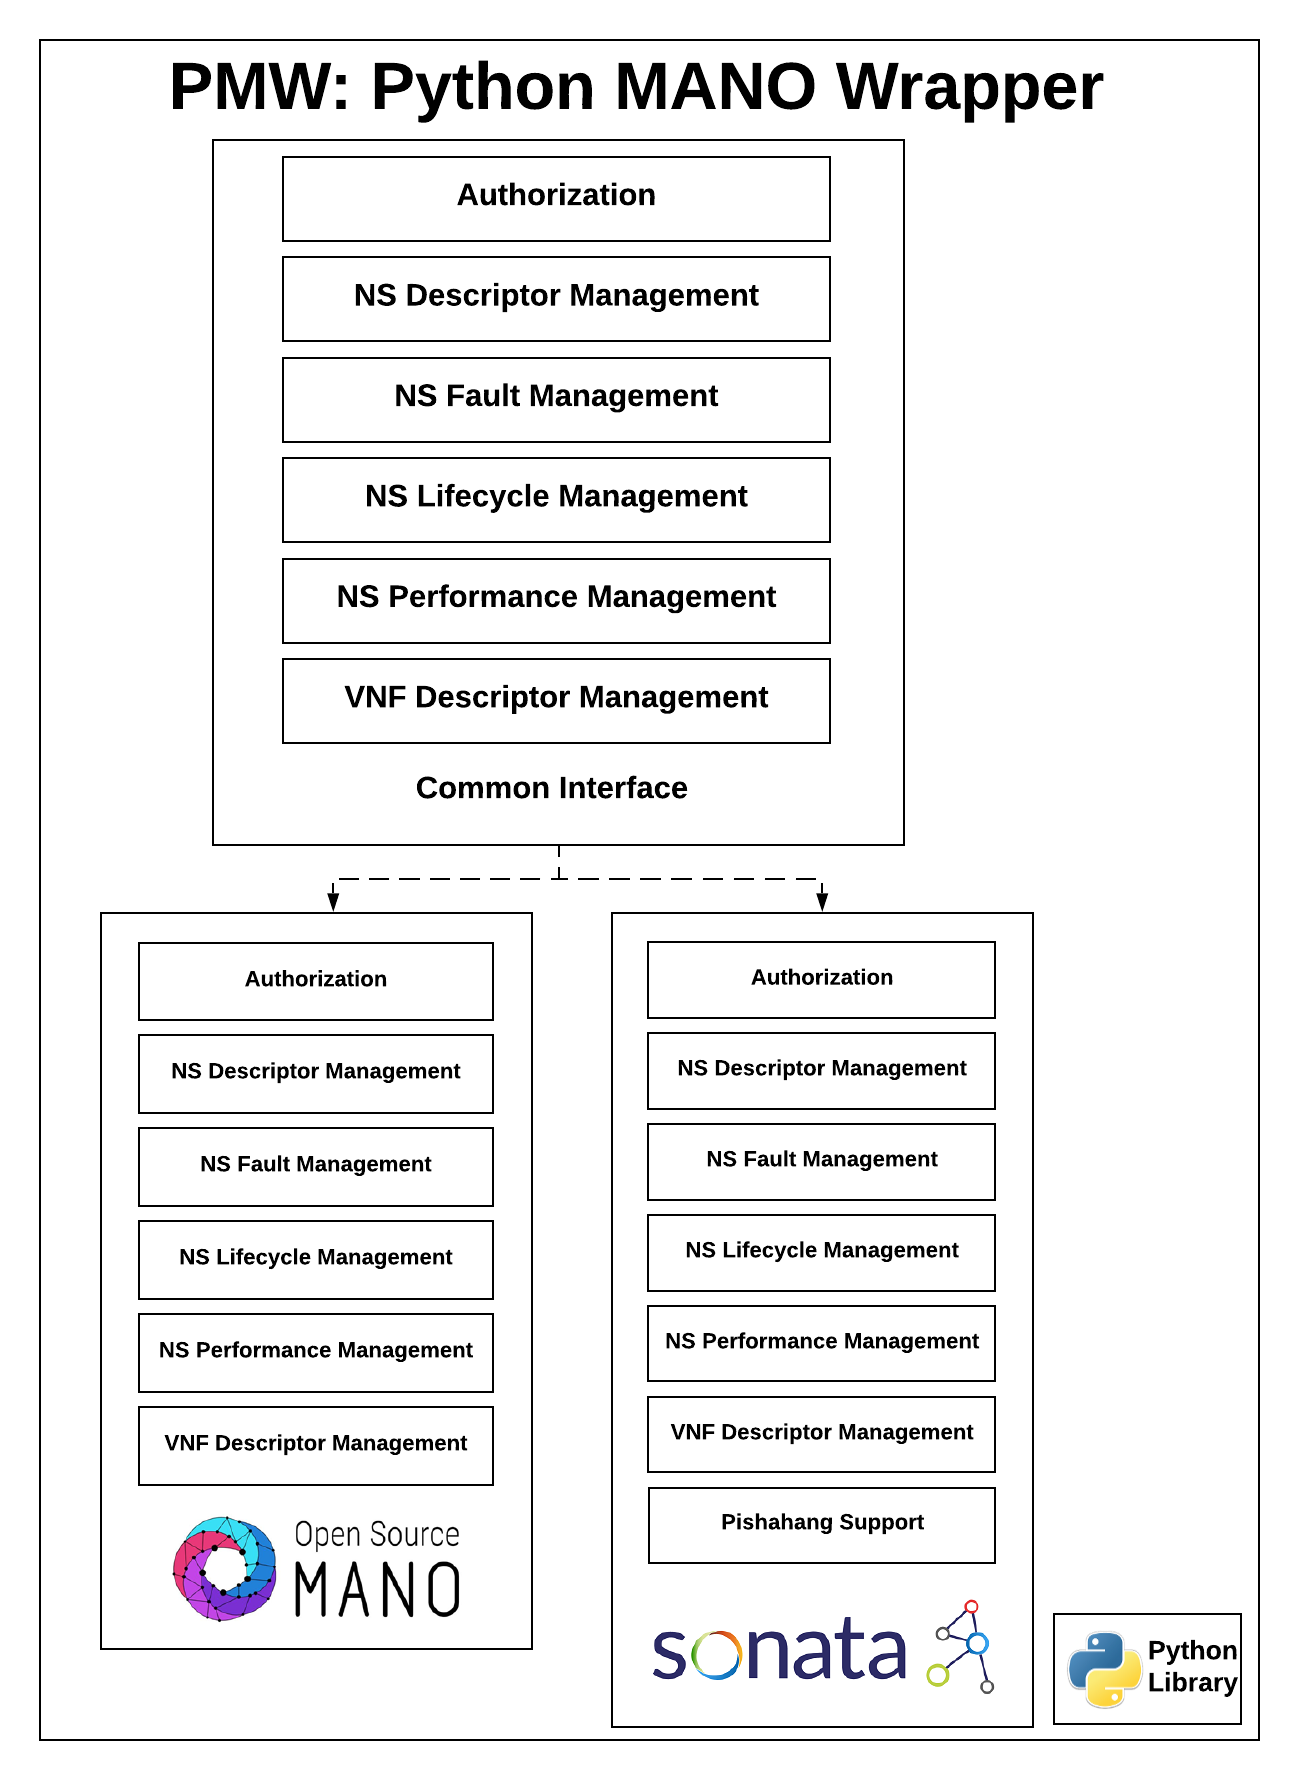
\includegraphics[width=1\linewidth]{figures/WrapperArch}
	\caption{PWM Common interfaces}
	\label{fig:wrapperarch}
\end{figure}

\begin{figure}
	\centering
	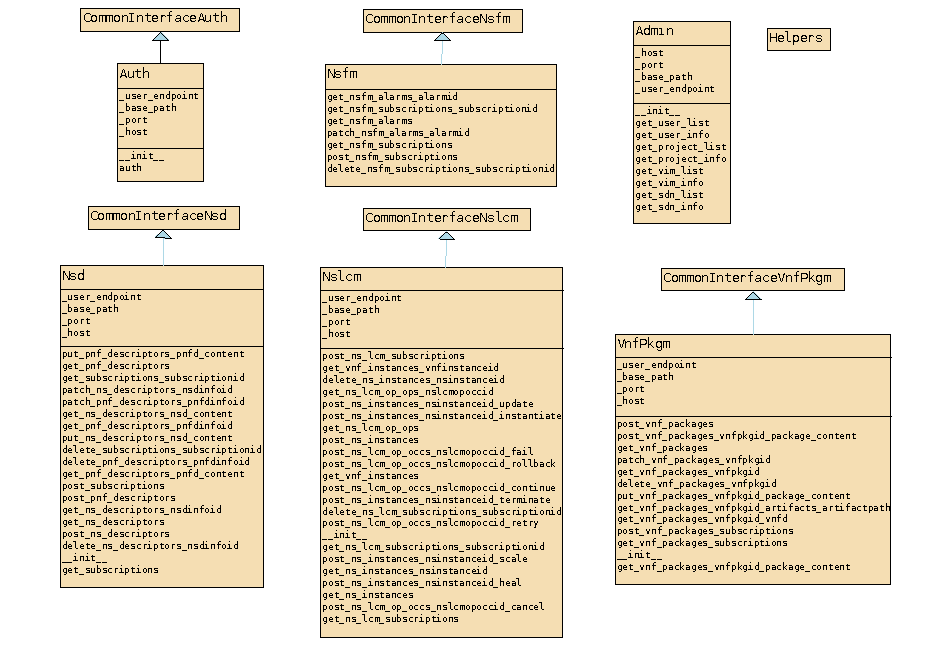
\includegraphics[width=1\linewidth]{figures/osm_class_diagram}
	\caption{OSM Wrappers implemented based on the CommonInterface base classes}
	\label{fig:osmclassdiagram}
\end{figure}

\begin{figure}
	\centering
	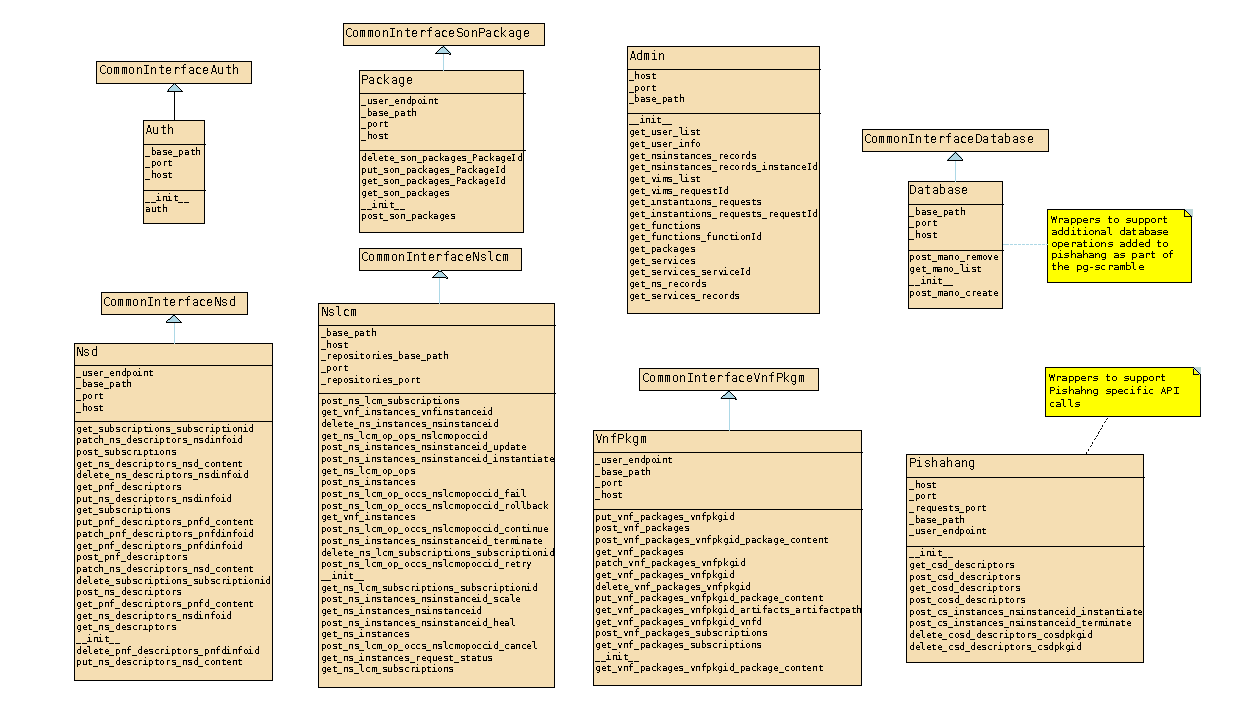
\includegraphics[width=1\linewidth]{figures/pishahang_class_diagram}
	\caption{Pishahang Wrappers implemented based on the CommonInterface base classes}
	\label{fig:osmclassdiagram}
\end{figure}


\subsection{Installation and usage}

PWM can be installed using pip by using this command \texttt{pip install python-mano-wrappers}. 

A simple script to get started with PWM is shown in the Listing \ref{lis:simpleauth}, here, the wrappers are imported and a client object is created according to the MANO type. 
Currently supported are OSM and Sonata. 
Such a client object can be used to make REST calls relevant to the MANO type. 
An example usage to retrieve all the network service descriptors of OSM can be seen from the listing \ref{lis:osmnsd}, here, the OSMClient module is used to first fetch an auth token and further using the auth token to fetch the relevant information, in this case NSD descriptors.


\begin{lstlisting}[caption=Simple wrapper code to fetch token, label=lis:simpleauth]
import wrappers

username = "admin"
password = "admin"
mano = "osm"
# mano = "sonata"
host = "osmmanodemo.com"

if mano == "osm":
	_client = wrappers.OSMClient.Auth(host)
elif mano == "sonata":
	_client = wrappers.SONATAClient.Auth(host)

response = _client.auth(
							username=username, password=password)

print(response)

\end{lstlisting}

\begin{lstlisting}[caption=Code to fetch all NSDs in OSM, label=lis:osmnsd]
import wrappers

osm_nsd = wrappers.OSMClient.Nsd(HOST_URL)
osm_auth = wrappers.OSMClient.Auth(HOST_URL)

_token = json.loads(osm_auth.auth(
									username=USERNAME,
									password=PASSWORD))

_token = json.loads(_token["data"])

response = json.loads(osm_nsd.get_ns_descriptors(
											token=_token["id"]))
response = json.loads(response["data"])
\end{lstlisting}

\subsection{Challenges}

Implementing such a python wrapper for a REST API is straight forward from the implementation perspective. 
However, the challenges that we faced are when identifying the required functional documentation from the respective MANOs. 
OSM and Sonata do not yet fully support the ETSI suggested endpoints and this combined with the lack of unified documentation, made it difficult in the begining to decide on the scope of supported functionalities.\\
  

\subsection{Future scope of wrappers}

PWM is built with easy maintanability and feature addition in mind. 
PWM makes it easy to add support for other MANOs. 
We expect MANO developers to use the common interface that we have suggested to add support to their REST APIs in python.

 


